% Chapter Template

\chapter{Development and Discussion} % Main chapter title

\label{Chapter4} % Change X to a consecutive number; for referencing this chapter elsewhere, use \ref{ChapterX}

%----------------------------------------------------------------------------------------
%	SECTION 1
%----------------------------------------------------------------------------------------

\section{Overview}

The first revision of the prototype case is presented in this chapter. 
Specifically, this section goes into detail about the process of designing as an iterative process where improvements and changes to the design are discussed and evaluated.


%----------------------------------------------------------------------------------------
%	SECTION 2
%----------------------------------------------------------------------------------------

\section{Initial Concepts}

At the initial stage of planning, multiple approaches to the MEGAphone chassis were conceptualised before making a final selection. 
Two of these designs incorporated ‘stands’ to prop the device up in order to minimise physical effort from the user, as well as all designs featuring a curved design to accommodate comfortable device holding for a large range of hand grip sizes. 
Each of these designs are outlined in the following sub-sections.

%-----------------------------------
%	SUBSECTION 1
%-----------------------------------
\subsection{Design One}

% LIST PROS AND CONS OF EACH DESIGN
% PERHAPS RANKING SYSTEM, EXPLAIN WHY DESIGN 3 WAS CHOSEN

Design ‘One’ as named was the first concept to be sketched using LibreCAD software. 
In hindsight, most of this design’s features are quite mundane in that while they account for all major ports and include a device stand to prop it up, in terms of the ergonomics, there are very few stand-out features. 
One thing that can be noted is that the case is compact with curved profile on either side where the user’s hands are expected to rest.

% \begin{figure}[hbt!]
% \centering
% 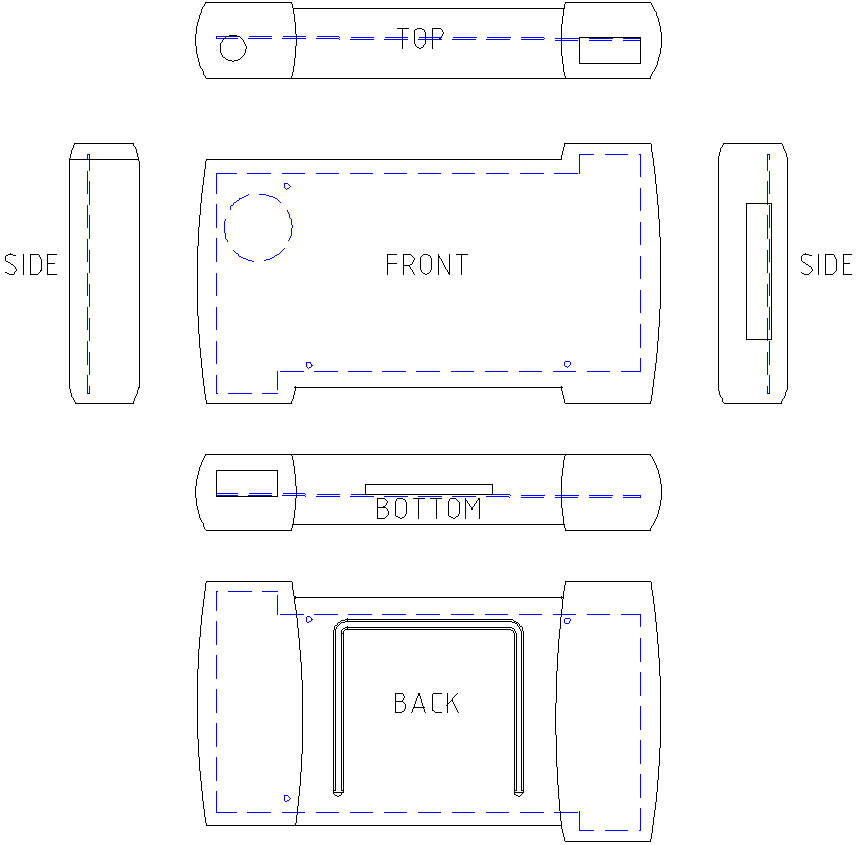
\includegraphics[width=10cm,height=10cm,keepaspectratio]{Figures/design1_sketch.png}
% \caption{This is a sketch of the first concept design drawn to scale of the PCB}
% \label{fig:Design_1}
% \end{figure}

%-----------------------------------
%	SUBSECTION 2
%-----------------------------------
\subsection{Design Two}

The second design was intended to mimic a video game controller in order to conform better to the hand as well as give users a more intuitive layout in regards to the orientation of the device when in use. 
UD and the MEGAphone project have two common traits in that they intend for the device to be simple, to use and to defend against security threats under the mantra ‘security through simplicity’ REF. 
This concept inhabits this trait arguably to the highest degree.

% \begin{figure}[hbt!]
% \centering
% 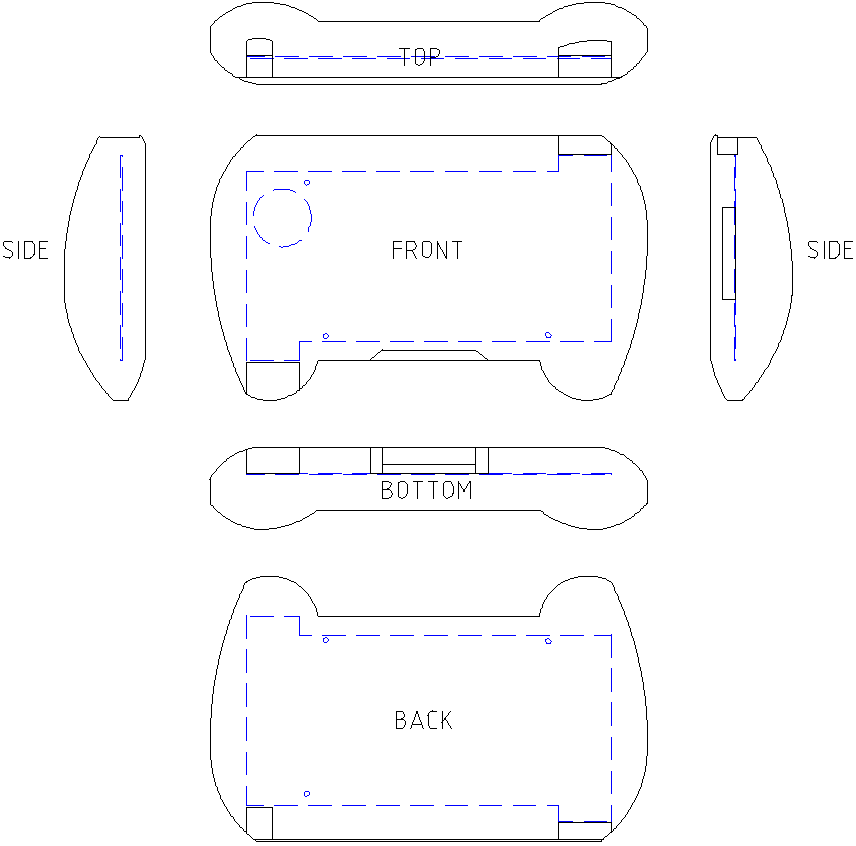
\includegraphics[width=10cm,height=10cm,keepaspectratio]{Figures/design2_sketch.png}
% \caption{This is a sketch of the second concept design drawn to scale of the PCB}
% \label{fig:Design_2}
% \end{figure}

%-----------------------------------
%	SUBSECTION 3
%-----------------------------------
\subsection{Design Three}

There were a few factors that made this design the final candidate in which to base the main deliverable of this project.
This approach uses handgrips to subconciously hint to the user the correct orientation to hold the device.
The use of a stand to prop the device up for extended periods of time was a useful addition as it reduces the amount of effort from the user, therefore reducing fatigue.

% \begin{figure}[hbt!]
% \centering
% 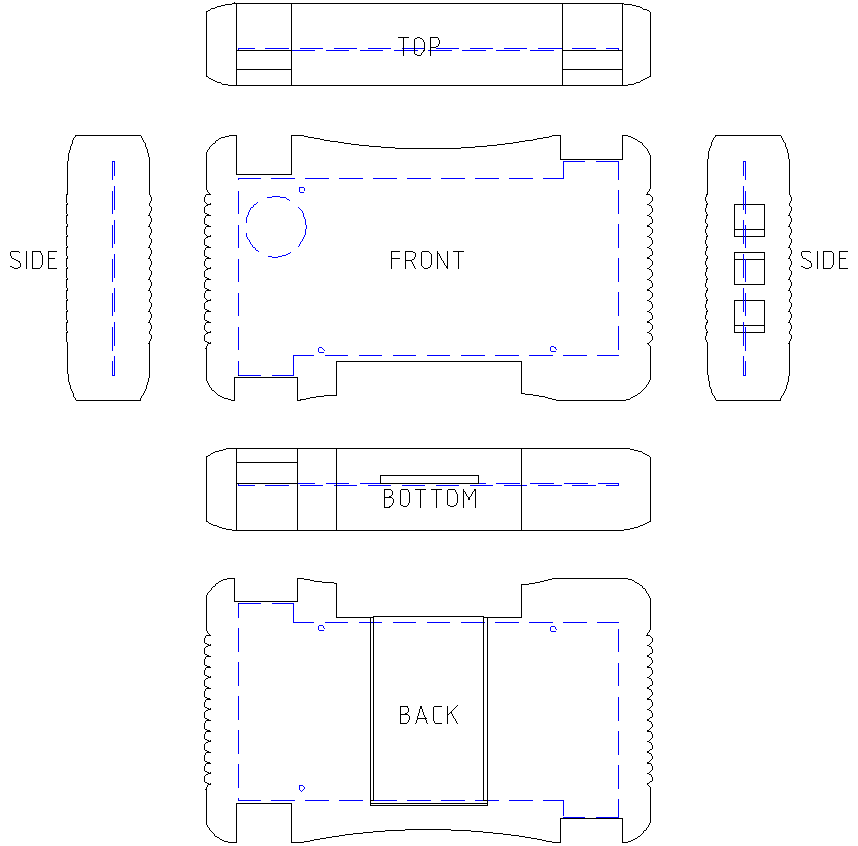
\includegraphics[width=10cm,height=10cm,keepaspectratio]{Figures/design3_sketch.png}
% \caption{This is a sketch of the third concept design drawn to scale of the PCB}
% \label{fig:Design_3}
% \end{figure}

%----------------------------------------------------------------------------------------
%	SECTION 3
%----------------------------------------------------------------------------------------

\section{First Revision}

The following section covers the development of all aspects of the accessible MEGAphone chassis as well as the accompanying hardware such as buttons or hinges.

%-----------------------------------
%	SUBSECTION 1
%-----------------------------------
\subsection{CAD Sketch}

The first stage of design after the initial concepts was the CAD sketching stage.
This was approached by beginning with a front view of the sketch where users would typically interact with the device, however just the outline was extruded outwards in order to create a tangible object in which to mold and add features later on in the process.


%-----------------------------------
%	SUBSECTION 2
%-----------------------------------
\subsection{Hand Grips}

The first stage of design after the initial concept sketches intended to use rubber grips on both sides of the device featuring a ridged pattern.
However, this concept was removed in favour of a ridges that resemble the size and shape of human adult fingers to more intuitively direct the user to hold the device in the correct fashion.
Another aspect that was considered since the early stages, while less obvious in the final product due to the curved nature, was the introduction of rounded corners as this would minimise hazards to the user.
This was also the case with other edges of the device, in that they were filleted at 1.5mm to remove the sharpness of the device.

% This was after receiving feedback from my supervisor following an initial design (show design, before and after).

%-----------------------------------
%	SUBSECTION 3
%-----------------------------------
\subsection{Rocker Switches}

A major issue that was identified from the start with the second revision PCB was that placement and size of switches made it difficult to access.
Larger rocker switches were chosen to be placed on the front surface above the screen as this is in full visability of the user during use.
The orientation of switches was completely intentional; for easier access for those with limited motor function or even without fingers, having the switches flip vertically would ensure that users are far less likely to flip wrong switch.
An earlier design incorporated the use of standoffs in the design in which to mount the PCB for the switches which was additionally included in the PCB design (view section 4.4). %fix this
This was however later removed as when soldered to the switch contacts, the PCB would hold in place without issue and adding those supports would just add weight and increase complexity.

%-----------------------------------
%	SUBSECTION 4
%-----------------------------------
\subsection{Jellybean Switch}

The Jellybean switch bought exclusively for this project interfaces with the device using a 3.5mm Audio Jack connector. 
Given that it is a single digital input device, hardware-implemented software accessibility capable of easily communicating with this device was relatively simple to implement. 
The second revision PCB during commencement of this project did not feature a working 3.5mm Jack connector, therefore, based on this knowledge, the 9-pin DSUB port of the device was hijacked as a single digital input under pin 7 for the Jellybean switch. 
The PCB ‘adapter’ created for this purpose is discussed in section 4.4. %fix this
This uses the same pin as the fire button on a retro Commodore64 Joystick controller, hence, integration into the MEGA65 operating system would be straightforward.

%-----------------------------------
%	SUBSECTION 5
%-----------------------------------
\subsection{Recessed Buttons}

% talk about recessing the buttons so that if the device is dropped, minimal/no accidental button presses are registered

One concept that improves the ‘quality of life’ of this product was the addition of recessed buttons.
There are potential situations where the device might be accidentally dropped and unintended button presses may be recorded where the addition of recessed buttons avoids or at least significantly reduces the risk of this situation.

This feature is designed around another existing constraint in that the PCB uses buttons that were repurposed from a Gameboy Advance. %%check this!
On the first prototype print, while allignment on the main MEGAphone PCB was correct, there was an issue regarding the clearance of the button cutout as well as the positioning of slots to hold the buttons in the correct orientation.


%-----------------------------------
%	SUBSECTION 6
%-----------------------------------
\subsection{3D-printed Prototype}

There was a significant issue that was overlooked with the first 3D printed prototype in that the thought behind orientation of components was flipped.
Electronic components (including connectors) needed more space underneath in order to fit comfortably and the design up until that point had not properly accounted for it.
The biggest issue was that the device ports were not thought of correctly.
The orientation of these ports is very important as this dictates how much volume each of the two main case components takes.
To rectify this issue, 

% so explain the process of rectifying this issue, map out the impacts and how they are resolved
% also add in that 0.15mm print resolution was used, not perfect as the project was very precise on top case in some parts, such as buttons, hence this should be done at higher resolution which means longer print time or silicone injection mould as a likely stronger, neater alternative

%-----------------------------------
%	SUBSECTION 7
%-----------------------------------
\subsection{Device Stand}

% thoughts behind the device stands, how they were conceptualised and why it was approached in such and such way; having two stands on either side adds to stability of the device as opposed to the original idea of having one stand in the middle, which also leaves space for solar panel in the middle
Originally the approach was to have a single stand oriented in the middle of the device where users could extend it out as they need.
However, having two stands on either end of the device has multiple advantages in that doing so increases the stability of the device, as well as gives ample space in the centre to place one or multiple solar panels depending on the available space (discussed in section 3.8).
The mechanism in which to extend and 'lock' the stand in place had the potential to be approached from a number of different angles.
One such angle that was a part of the final prototype was to have a sliding..

%-----------------------------------
%	SUBSECTION 8
%-----------------------------------
\subsection{Solar Panels}

% choice of solar panels, discuss potential options and why a specific one was chosen, do a table comparison of available panels and again explain the power output and cost etc.

%-----------------------------------
%	SUBSECTION 9
%-----------------------------------
\subsection{Device Strap / Key-chain}

% talk about process of designing this feature, how original design changed in favour of larger slot/strap for easier carry
The thought behind the key-chain feature of the device was to be able to clip it to things, and while this feature did see an appearance in an early prototype, it was later adapted into a 'housing' for an arm strap, to allow for easier carrying.
An extra notch was added to lock into the top part of the case and re-enforce the strength. 
The original prototype did not have this and as the length of the strap was extended, this was a consideration for supporting the weight of the device.

%-----------------------------------
%	SUBSECTION 10
%-----------------------------------
\subsection{Easy Access Keys}

The easy access keys were designed around the 'Nav Keys' developed by Storm Interface. %double check
They feature an array of easily distingishable keys which were inspired for this adaptation. 
It was first approached as an extension of the device as this would free up a lot of non-existent space.
However, it was ideal for the array of buttons to be integrated into the device as this ensures that the full extent of accessibility is available from the moment the device is picked up.
Due to the height requirement of the MEGAphone PCB, there was very little space to attach a slave PCB to allow button functionality, hence why there is an elevation in the button housing.
Additionally, there needed to be enough depth so that the PCB could be screwed into place comfortably.

An issue that came up in the first prototype print is that the keys did not have enough clearance to actuate without resistance.
This was fixed in the update by extending the width of the button cutouts by approximately 0.25mm. % check this

% FIXED AB AND DIRECTIONAL BUTTON SIZE CLEARANCE, ALSO EZ KEY CLEARANCE
% FIXED ALIGNMENT OF THROUGH HOLE

%-----------------------------------
%	SUBSECTION 11
%-----------------------------------
\subsection{Ventilation}

% device only uses about 1-2W of power, FPGA using 0.2W
% Not necessary in final design but add images of version with vents
Thermal management is a concept that came up later in the process as the MEGAphone device is a low power device by mobile device standards.
In its entirety, the device uses approximately 1-2W of power with the heart of the device, the FPGA, using about 0.2W of power.
This yields very little thermal output with the more notable power drawing components being the 110db speaker [source] and full colour 480p display [source].

%-----------------------------------
%	SUBSECTION 12
%-----------------------------------
\subsection{Potentiometers}

% Slide pot better than thumb wheel pot, explain about physical effort etc.
The potentiometer feature used to control aspects such as speaker volume was a feature that was omitted from the final design due to another more important requirement being the implimentation of EZ keys.
This is a feature that can be implemented by other means such as through the EZ keys themselves and therefore a prototype without this would not be a major issue.
A possible solution for this would be to employ an array of variable resistors as this would be the easiest in terms of the amount of effort that users have to extert.
Alternatively, any potentiometer that is too small or requires a twisting motion would be more difficult for some users, such as elderly users with weak grip strength.

%-----------------------------------
%	SUBSECTION 13
%-----------------------------------
\subsection{Port Access}

Port access was intentionally designed to have no case material on the top and bottom of the device as this would interfere with the plugging in of various peripherals.

An issue that was faced in the original prototype was in regard to the orientation of the port cutouts in that they were placed on the display side of the PCB.
This was rectified by extending out the bottom chassis component with the port cutout on that side so that it would match up with the true orientation of the ports. %expand on this later with images

%----------------------------------------------------------------------------------------
%	SECTION 4
%----------------------------------------------------------------------------------------

\section{PCB Design}
This section discusses the process in designing the supporting PCBs for this project.

% explain workaround for previous button layout, using slave boards with tactile switches as well as choice behind contact pads instead of connectors to save space

%-----------------------------------
%	SUBSECTION 1
%-----------------------------------
\subsection{Rocker Switch PCB}

The PCB designed to organise the routing of power to the array of rocker switches originally had the intention of interfacing with the main PCB through a connector of some sort.
Space has been limited however, therefore leading to an alternate solution in that there were 'mounting' pads to serve as a soldering point for the wires that would be routed to the main PCB.
An issue with the footprint that was observed after sourcing these parts, was that there was not enough clearance for the pins to 'slot' through.
The approach was to file down the pins on the rocker switches individually so that they would fit, which was not an issue in regards to current as the whole device runs on about 1-2W.
Filing down the PCB through-hole cutout would have been worse as there was potential for solder to not flow evenly due to damaging the solder mask. %double check this

During the case design process, having mounting points to hold the circuit board in place was considered.
This was later removed as the switches mount very securely in their cutouts, and the clearance between the PCB and the main MEGAphone PCB is very minimal.
This would allow adjustment if needed before soldering as well as making the repair process easier if users need to replace or modify certain parts.


%-----------------------------------
%	SUBSECTION 2
%-----------------------------------
\subsection{Easy Keys and Power}

The purpose behind the easy keys is to give users a platform in which to interact with the MEGAphone device while being as clear and easy to use as possible.
Multi-coloured, multi-shaped keys are employed make things as unambiguous as possible which include, left and right (forward and backward), up and down, and a 'fire' or enter key.
This is inspired by the Storm Nav-pad, where a version has been acheived to a budget, for the purpose of prototyping.

An important aspect of this device is to provide easy access to the power switch as turning the display on an off on this device is frequent due to not having automatic display toggle features.
This is intergrated into the device in the same manner as the easy keys, in that they work by momentarily pressing a tactile switch.
This interface faced an issue where the openings for the button cutouts were virtually the same size leading to problems with clearance. 
To fix this issue, the openings were extended by about half a millimetre on all sides to allow for smooth button pressing while still sitting securely in place.

%-----------------------------------
%	SUBSECTION 3
%-----------------------------------
\subsection{Audio Jack Adapter}

The audio jack adapter was designed to be a substitute for the original audio jack, which was unoperational at the time.
This PCB hijacks the fire pin of the 9-pin DSUB connector in order to 'imitate' a joystick fire button, coupled with hardware implemented features in the FPGA, the MEGAphone should treat any input as a regular device.
An issue that was faced was in regard to the overall size and shape of the PCB.
This was not thought about correctly at the time of manufacturing as the PCB was too bulky on either side and due to the central placement of the audio jack input, interfacing with this adapter was less than convienient.
To fix this, a nibbler was used to clip away at the edges to cut the board down to size, followed by a rough 80 grit sanding to smooth the edges somewhat.
Given that fibreglass particles are not good for health when inhaled, this was undertaken responsibly to ensure that these risks were avoided.

%----------------------------------------------------------------------------------------
%	SECTION 5
%----------------------------------------------------------------------------------------

\section{PCB Layout}

% analyse the changes in the final design, what limitations the existing PCB layout has and propose a better layout that satisfies the UD principles, talk about what is ideal and what is the best that can be done with current layout. 
% Ideal layout includes ports at top of device along with rocker switches replacing current rev2 switches on the main PCB

%-----------------------------------
%	SUBSECTION 1
%-----------------------------------
\subsection{Original Design}

The layout of the second revision MEGAphone PCB served as the major constraint of this project, as the case design had to be designed around it without any significant redesign due to the complexity of the device. Certain reworks to better adapt the design to an accessible interface included removing the existing switches in favour of larger rocker switches hosted on an external PCB (VIEW).

%-----------------------------------
%	SUBSECTION 2
%-----------------------------------
\subsection{Proposed Design}

A possible solution to the existing PCB which does inhabit the Universal Design principles is proposed in FIGURE. 
The underlying idea with this redesign was to integrate the design all onto one PCB. Doing so would reduce the amount of wires required and given that those in the current solution are soldered to make space, it makes the design overall ‘simpler’.

In order to make the device more intuitive, placement of the 9-pin DSUB port should be moved to the ‘top’ of the device in the same orientation as the VGA port, so that users know from a glance that this is where all device ports are expected to be.
The accessible button interface also utilises an external PCB which hosts the tactile switches that were opted to form the base of the accessible button function. 
Other options were considered, such as silicone rubber pads, as used for the directional button and ‘A’, ‘B’ buttons. However, due to the nature of the


%----------------------------------------------------------------------------------------
%	SECTION 6
%----------------------------------------------------------------------------------------

\section{Software}

% talk about keyboard accessibility, term ‘android accessibility encapsulation’ discuss this.
% Also mention program is working in parallel to the software ‘mimicking’ the c64 system so this is not a C program running on MEGA65 but rather VDHL, a hardware description language

%-----------------------------------
%	SUBSECTION 1
%-----------------------------------
\subsection{Accessible Keyboard}

Nunc posuere quam at lectus tristique eu ultrices augue venenatis.

%-----------------------------------
%	SUBSECTION 2
%-----------------------------------
\subsection{PART2}

Nunc posuere quam at lectus tristique eu ultrices augue venenatis.

%-----------------------------------
%	SUBSECTION 3
%-----------------------------------
\subsection{PART3}

Nunc posuere quam at lectus tristique eu ultrices augue venenatis.

%----------------------------------------------------------------------------------------
%	SECTION 7
%----------------------------------------------------------------------------------------

\section{Summary}

Lorem ipsum dolor sit amet, consectetur adipiscing elit.